% HIKET -- storyline working note for coauthors.
% A mid-tier document between the figure storyboard and the manuscript: the argument
% read as one flowing story, with the figures AND tables it rests on. No methods,
% no full literature -- a testbed to feel how the story punches and where it lands.
% (Narrative-craft scaffolding is applied but deliberately not surfaced in the text.)
\documentclass[11pt]{article}
\usepackage[utf8]{inputenc}\usepackage[T1]{fontenc}
\usepackage[margin=2.4cm]{geometry}
\usepackage{graphicx}\usepackage{amsmath}\usepackage{xcolor}
\usepackage{float}\usepackage[hidelinks]{hyperref}
\usepackage{tikz}\usetikzlibrary{positioning, arrows.meta, calc, fit, backgrounds}
\usepackage{caption}\captionsetup{font=small,labelfont=bf}
\usepackage[most]{tcolorbox}

% Methodological note box (a light-blue "reading note", visually distinct from the figures)
\definecolor{notebg}{HTML}{EAF2FB}\definecolor{noterule}{HTML}{2C6FB5}
\newtcolorbox{methodnote}{colback=notebg, colframe=noterule, boxrule=0pt, leftrule=3pt,
  arc=1pt, left=8pt, right=8pt, top=5pt, bottom=5pt, fontupper=\small,
  before skip=8pt, after skip=8pt}

\newcommand{\sinit}{\sigma_{\mathrm{init}}}
\newcommand{\sinput}{\sigma_{\mathrm{input}}}
\newcommand{\fig}{figures}
\newcommand{\mm}{../Calibration_real_data_transient/diagnostics/multimodel}
\newcommand{\rep}{../Reporting/NextgenC_report}

\title{\vspace{-1.4cm}\textbf{HIKET --- the storyline}\\[2pt]
\large a working note for coauthors}
\author{}
\date{\small Version of \today\ --- a narrative testbed, not the manuscript.
No methods or full referencing; the point is to read the argument whole and see how it flows.}

\begin{document}
\maketitle

% ---------------------------------------------------------------------------
% STATUS BLOCK inserted 2026-08-10. Delete once the run below has landed and
% the affected passages have been rewritten.
% ---------------------------------------------------------------------------
\begin{center}
\fbox{\begin{minipage}{0.93\textwidth}
\small
\textbf{DRAFT STATUS --- 2026-08-10.} All figures and numbers in this note are keyed to the
\texttt{20260807\_1655*} posteriors and are \textbf{provisional}. A recalibration is in flight
(Roihu jobs 563524--563529, commit \texttt{3b0d533}) which corrects the likelihood error scale,
the Fortran precision of Yasso15/20, and three prior widths misread from their sources. Two
findings that will need incorporating either way:
\textbf{TP3's non-convergence is a result, not a defect} --- its two modes fit within 4.2 nats, so
the third pool is not identifiable from two SOC observations per plot; and
\textbf{bulk residence times must be quoted from the intrinsic basis}
(\texttt{doublechecks/intrinsic\_mrt.R}), not from the earlier contaminated computation.
\end{minipage}}
\end{center}

\vspace{-0.6cm}

\noindent\textbf{What this is.} Below is the HIKET argument told as one continuous story,
with each figure and table placed where the story needs it. It follows an
Opening--Challenge--Action--Resolution arc with three side threads; the schema on the
next page is the map. The prose is deliberately compact --- enough to feel the flow and
judge whether it lands --- and is the scaffold the manuscript will be written onto.

% =====================================================================
\section*{The story at a glance}

\begin{center}\small
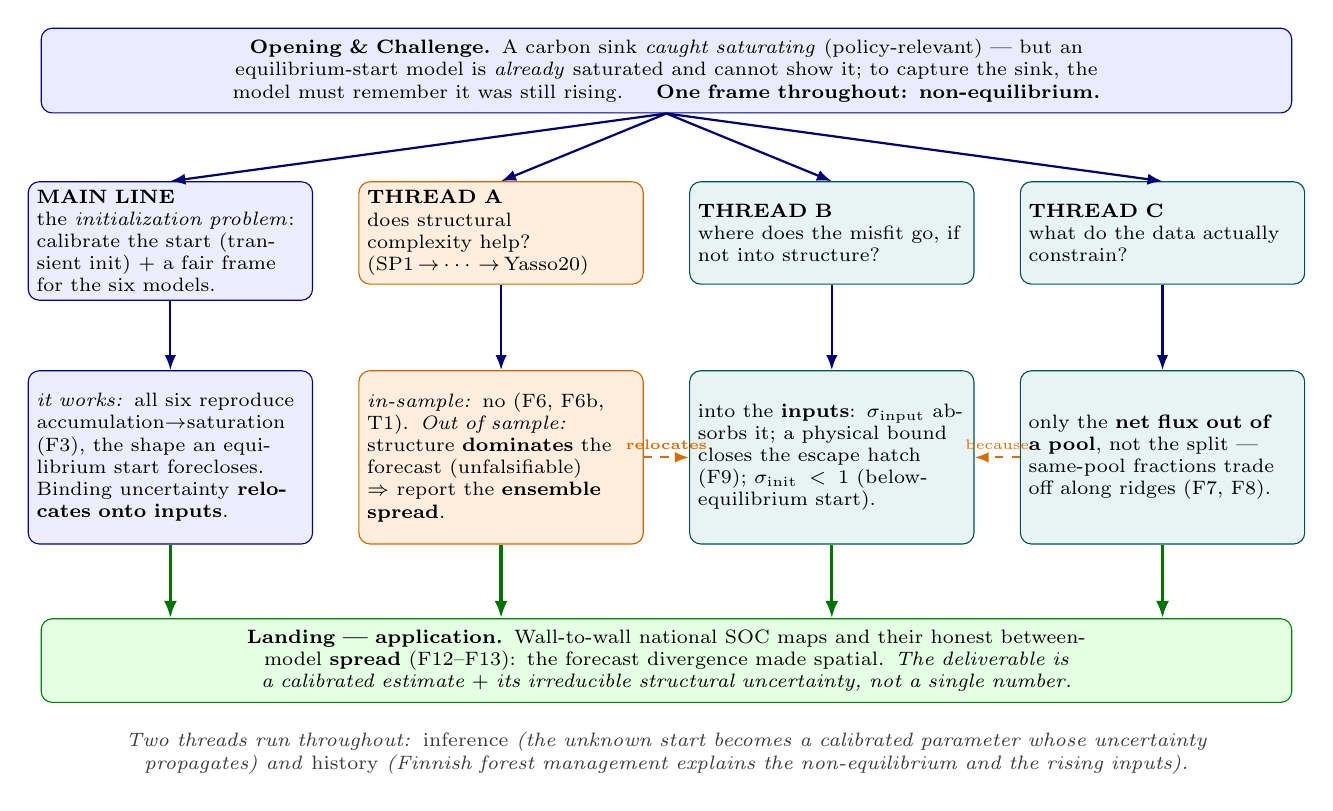
\begin{tikzpicture}[
  font=\scriptsize,
  prem/.style={rectangle, rounded corners, draw=blue!55!black, fill=blue!8, align=center,
               text width=156mm, inner sep=4pt},
  setb/.style={rectangle, rounded corners, align=left, text width=34mm, inner sep=3pt, minimum height=13mm},
  payb/.style={rectangle, rounded corners, align=left, text width=34mm, inner sep=3pt, minimum height=22mm},
  mc/.style={draw=blue!55!black, fill=blue!7},
  ac/.style={draw=orange!80!black, fill=orange!13},
  tc/.style={draw=teal!65!black, fill=teal!9},
  land/.style={rectangle, rounded corners, draw=green!50!black, fill=green!10, align=center,
               text width=156mm, inner sep=4pt},
  dn/.style={-{Latex[length=1.9mm]}, thick, blue!45!black},
  cv/.style={-{Latex[length=2.2mm]}, very thick, green!45!black},
  hz/.style={-{Latex[length=1.8mm]}, thick, dashed, orange!85!black}]
\def\ca{0}\def\cb{4.2}\def\cc{8.4}\def\cd{12.6}
\node[prem, anchor=north] (P) at (6.3,0)
  {\textbf{Opening \& Challenge.} A carbon sink \emph{caught saturating} (policy-relevant) --- but an equilibrium-start
   model is \emph{already} saturated and cannot show it; to capture the sink, the model must remember it was still
   rising. \quad\textbf{One frame throughout: non-equilibrium.}};
% --- row 1: each arc's setup ---
\node[setb, mc, anchor=north] (M1) at (\ca,-1.95) {\textbf{MAIN LINE}\\ the \emph{initialization problem}: calibrate the start (transient init) + a fair frame for the six models.};
\node[setb, ac, anchor=north] (A1) at (\cb,-1.95) {\textbf{THREAD A}\\ does structural complexity help? (SP1\,$\to$\,$\cdots$\,$\to$\,Yasso20)};
\node[setb, tc, anchor=north] (B1) at (\cc,-1.95) {\textbf{THREAD B}\\ where does the misfit go, if not into structure?};
\node[setb, tc, anchor=north] (C1) at (\cd,-1.95) {\textbf{THREAD C}\\ what do the data actually constrain?};
% --- row 2: each arc's resolution (aligned) ---
\node[payb, mc, anchor=north] (M2) at (\ca,-4.35) {\emph{it works:} all six reproduce accumulation$\to$saturation (F3), the shape an equilibrium start forecloses. Binding uncertainty \textbf{relocates onto inputs}.};
\node[payb, ac, anchor=north] (A2) at (\cb,-4.35) {\emph{in-sample:} no (F6, F6b, T1). \emph{Out of sample:} structure \textbf{dominates} the forecast (unfalsifiable) $\Rightarrow$ report the \textbf{ensemble spread}.};
\node[payb, tc, anchor=north] (B2) at (\cc,-4.35) {into the \textbf{inputs}: $\sinput$ absorbs it; a physical bound closes the escape hatch (F9); $\sinit<1$ (below-equilibrium start).};
\node[payb, tc, anchor=north] (C2) at (\cd,-4.35) {only the \textbf{net flux out of a pool}, not the split --- same-pool fractions trade off along ridges (F7, F8).};
% --- landing ---
\node[land, anchor=north] (L) at (6.3,-7.5)
  {\textbf{Landing --- application.} Wall-to-wall national SOC maps and their honest between-model \textbf{spread}
   (F12--F13): the forecast divergence made spatial. \emph{The deliverable is a calibrated estimate $+$ its
   irreducible structural uncertainty, not a single number.}};
% arrows
\foreach \n in {M1,A1,B1,C1} \draw[dn] (P.south) -- (\n.north);
\foreach \s/\p in {M1/M2,A1/A2,B1/B2,C1/C2} \draw[dn] (\s) -- (\p);
\foreach \p in {M2,A2,B2,C2} \draw[cv] (\p.south) -- (\p.south |- L.north);
\draw[hz] (A2.east) -- node[above=-0.3mm, font=\tiny\bfseries]{relocates} (B2.west);
\draw[hz] (C2.west) -- node[above=-0.3mm, font=\tiny]{because} (B2.east);
\node[below=2.5mm of L, text width=156mm, align=center, font=\scriptsize\itshape, gray!45!black]
  {Two threads run throughout: \emph{inference} (the unknown start becomes a calibrated parameter whose uncertainty
   propagates) and \emph{history} (Finnish forest management explains the non-equilibrium and the rising inputs).};
\end{tikzpicture}
\end{center}

\noindent The through-line is one physical fact --- \textbf{these soils are not at equilibrium} --- seen from two
sides: it is why there is a sink to report (the stakes) and why a conventional model cannot show it (the obstacle).
The whole paper is the work of turning the second into a solution for the first.

% =====================================================================
\section{Opening: a sink caught saturating, and a model that cannot see it}

Finnish forest soils have been accumulating carbon through the observation period and are now bending toward a
plateau. This incipient saturation is not a modelling curiosity: Finland reports it in its national greenhouse-gas
inventory, where most countries assume a flat soil pool, so getting it right has direct policy weight. The signal
has a physical cause. Across the twentieth century the country's forests recovered from a depleted, heavily-used
early-century base, and the growing stock has risen by roughly seventy percent since the 1970s
(Fig.~\ref{fig:history}); the litter those forests return to the soil rose with them and then levelled off, and it
varies strongly from south to north (Fig.~\ref{fig:inputs}). A rising, non-stationary input history feeding soils
that were well below their carrying capacity is exactly the setup for an accumulating, saturating sink.

\begin{figure}[htbp]\centering

\includegraphics[width=0.86\linewidth]{\fig/F10b_forest_history.png}
\caption{\textbf{The non-equilibrium premise.} National growing stock (NFI, 1921--2023): a depleted, near-stationary
base into the 1970s, then a sustained recovery. The 1917 pre-initialisation anchor and the two SOC campaigns are
marked. Source: Korhonen, R\"aty et al.\ (2024).}\label{fig:history}
\end{figure}

\begin{figure}[htbp]\centering

\includegraphics[width=0.86\linewidth]{\fig/F1_inputs.png}
\caption{\textbf{The inputs.} Litter forcing over time (composition; a rise to a mid-2000s peak, then a plateau)
and its strong south--north gradient, with climate shown only as context. The accumulation is input- and
history-driven, and the inputs vary enormously in space.}\label{fig:inputs}
\end{figure}

The trap is that a soil model run the conventional way cannot represent any of this. Started at steady state --- the
near-universal default --- the model already sits at its saturated end-state, with nowhere left to accumulate. Run
forward at published parameters from an equilibrium start, it stays flat, and well below the observed stocks
(Fig.~\ref{fig:baseline}). The very phenomenon we most want to capture is the one the standard convention forecloses.

\begin{figure}[htbp]\centering

\includegraphics[width=0.78\linewidth]{\fig/F2_baseline.png}
\caption{\textbf{The trap.} Yasso20 at published defaults with an equilibrium start, averaged over all plots: flat,
because an equilibrium start cannot accumulate, and low relative to the observed campaign means.}\label{fig:baseline}
\end{figure}

% =====================================================================
\section{Challenge: to show the saturation, the model must remember it was still rising}

The stakes and the obstacle are the same fact from two sides. The soils hold an accumulating sink \emph{because}
they are out of equilibrium; the standard model fails \emph{because} it assumes they are not. So capturing the
observed dynamic is not a matter of better parameters --- it requires abandoning the equilibrium-start convention and
initialising the model as a system still recovering from its history. That is the initialization problem, and it is
the axis the whole study turns on: how do you start a non-equilibrium simulation when you have no record of the
forcing that produced the initial state?

% =====================================================================
\section{Action: transient initialization under a fair frame}

The move is to stop \emph{assuming} the initial state and instead \emph{calibrate} it. Each model is spun up from a
below-equilibrium historical anchor to the start of the observation period, and the initial carbon becomes a
calibrated quantity, $\sinit$, whose uncertainty propagates into both the starting state and the forward run rather
than being fixed by fiat. Casting the unknown start as an inferred parameter, not a fixed assumption, is what makes
this tractable at scale.

The comparison across models only means something if the models are not secretly competing on who guessed the inputs
or the initial state best. We therefore put all six on an even footing: homogenised priors (identical in
construction, not in raw number), equal degrees of freedom in the inter-pool flow fractions, and two auxiliary
parameters --- $\sinit$ for the initial state and $\sinput$ for the litter level --- that absorb init- and
input-uncertainty identically for every model. The six span a deliberate complexity ladder: a one-pool model (SP1),
two- and three-pool cascades (TP2, TP3), and the three five-pool Yasso variants, with a second, climate-integration
axis running Yasso07~$\to$~15~$\to$~20. On this even ground, structure --- and only structure --- is what varies.

% =====================================================================
\section{Resolution: it works, and the binding uncertainty relocates}

\subsection{The payoff}
Transiently initialised, all six models reproduce the observed shape --- accumulation bending toward incipient
saturation --- and track the later campaign means (Fig.~\ref{fig:meansoc}). This is the shape an equilibrium start
cannot produce: solving the initialization problem is precisely what lets the models represent the policy-relevant
sink. The payoff comes with an honest caveat visible in the reconstructed trajectory
(Fig.~\ref{fig:init}): the models converge on a 1985 stock some 26~tC\,ha$^{-1}$ above the observed start, a
consequence of the coarse, unrecorded pre-1985 phase --- a live question, not a failure of the method.

\begin{methodnote}
\textbf{Reading note --- the SOC observations have been rebuilt; these figures predate the rebuild.}
The campaign points in this and the next figure are \emph{whole-profile} carbon --- organic layer plus mineral soil,
not the 0--40\,cm inventory total --- but they were produced from our earlier SOC assembly, which we have since
replaced. Two defects were found (2026-08-03) and corrected. First, the mineral layers carried no coarse-fragment
(stoniness) correction, which inflated mineral carbon by a near-constant factor of $\approx$1.6; with a median
stoniness of 43\%, $1/(1-0.43)$ accounts for it. Second, the three campaigns were processed along separate paths
that had drifted apart, so part of the 1985$\to$2006 change was protocol rather than dynamics.

All three campaigns now come from one LUKE source (organic $+$ mineral, stoniness- and bulk-density-corrected),
reproducing the official national stocks exactly, with the deep tail extrapolated per plot only as far as augering
actually reached rather than to a flat 1\,m. The corrected target rises gently --- campaign medians 59.4, 66.7,
67.4\,tC\,ha$^{-1}$ --- where the old one gave 63, 102, 105, i.e.\ a 62\% jump between 1985 and 2006 that was an
artefact. Section~\ref{sec:socdata} of the main manuscript documents this in full.

\smallskip
\noindent\textbf{What this means for the figures below.} They stand as the argument's \emph{shape} --- the
accumulation-then-saturation, the model ordering, the initialization gap --- but their SOC levels, and any number
quoted against a campaign mean (including the 26\,tC\,ha$^{-1}$ 1985 offset above), are tied to the superseded
target and will be restated once the six models are recalibrated on the corrected data. Read the levels as
provisional; read the structure as the result.
\end{methodnote}

\begin{figure}[htbp]\centering

\includegraphics[width=0.80\linewidth]{\fig/F3_mean_soc.png}
\caption{\textbf{The central result.} Cross-plot mean SOC, all six models, 1985--2024: rise then bend toward
saturation, tracking the Biosoil/Komeetta campaign means. Colour runs from the simple models (green) to the Yasso
family (warm).}\label{fig:meansoc}
\end{figure}

\begin{methodnote}
\textbf{Reading note --- depth basis.} As in Fig.~\ref{fig:meansoc}, the observed campaign stocks (panel a) are
whole-profile values (measured organic $+$ 0--40\,cm, plus a modelled deep tail), and they too come from the
superseded SOC assembly described in the note above. Levels provisional, structure robust.
\end{methodnote}

\begin{figure}[htbp]\centering

\includegraphics[width=0.98\linewidth]{\fig/F4_initialization.png}
\caption{\textbf{The initialization problem, made visible.} (a) The full trajectory including the reconstructed
transient-init spin-up 1917$\to$1985 and the observed window; the models recover from a below-equilibrium start but
disagree about how much, and all reach $\sim$26~tC\,ha$^{-1}$ above the observed 1985 stock. (b) The future forecast
2025$\to$2084: agreement where calibrated, sharp divergence when extrapolated.}\label{fig:init}
\end{figure}

\subsection{Thread A --- does adding structural complexity improve the answer?}
In-sample, no. Predictive skill does not climb the pool ladder or the climate sub-axis; the most complex model
fits worst, on both calibration and independent holdout (Fig.~\ref{fig:skill}, Fig.~\ref{fig:complexity}). We do
make the anti-complexity claim, but scope-bounded: for an applied, recalibratable, single-region task whose aim is
accuracy plus calibrated uncertainty, added structure does not buy skill and can cost it. That is not a verdict on
Yasso, which is optimised for a different objective --- generality, standardisation, and litter-quality resolution
that this single-region fit test simply does not measure --- so ``more complexity does not help \emph{here}'' and
``Yasso is the right inventory tool'' coexist. Table~\ref{tab:summary} is the whole comparison at a glance.

\begin{figure}[htbp]\centering

\includegraphics[width=0.98\linewidth]{\fig/F6_obs_vs_pred_holdout.png}
\caption{\textbf{Skill on the honest set.} Observed vs.\ predicted SOC on the held-out plots, by model, with points
classed by stand basal-area quintile. Skill is uniformly low and the ranking nearly collapses out of sample; the
red least-squares line is far flatter than the 1:1 dashed line (the models compress the range).}\label{fig:skill}
\end{figure}

\begin{figure}[htbp]\centering

\includegraphics[width=0.90\linewidth]{\fig/F6b_skill_vs_complexity.png}
\caption{\textbf{Complexity does not move the answer.} Predictive $R^2$ against structural complexity: the pool-axis
slope is negative and the climate sub-axis falls monotonically; the most complex model is the worst on both
calibration and holdout.}\label{fig:complexity}
\end{figure}

\begin{table}[htbp]\centering
\caption{\textbf{Results at a glance.} Per-model structural complexity (pools, free parameters), skill ($R^2$
calibration and holdout, holdout RMSE), the input story (effective litter flux $\sinput\bar J$, all inside the
physical $[0.5,8.7]$~tC\,ha$^{-1}$\,yr$^{-1}$ envelope), and the initial state ($\sinit<1$). Complexity climbs while
skill does not.}\label{tab:summary}
% auto-generated by build_T1_model_summary.R -- per-model summary
\begin{tabular}{lccccccc}
\hline
Model & Pools & Free & $R^2$ & $R^2$ & RMSE & Eff.\ flux & $\sigma_{\mathrm{init}}$ \\
 & & params & (cal) & (hold) & (hold) & $\sigma_{\mathrm{inp}}\bar J$ & \\
\hline
SP1 & 1 & 6 & 0.017 & 0.000 & 46 & 4.9 & 0.67 \\
TP2 & 2 & 7 & 0.018 & 0.000 & 47 & 6.4 & 0.40 \\
TP3 & 3 & 9 & 0.019 & 0.000 & 47 & 6.5 & 0.37 \\
Yasso07 & 5 & 20 & 0.028 & 0.002 & 45 & 6.6 & 0.24 \\
Yasso15 & 5 & 26 & 0.031 & 0.004 & 44 & 5.9 & 0.18 \\
Yasso20 & 5 & 26 & 0.023 & 0.001 & 45 & 6.6 & 0.21 \\
\hline
\end{tabular}

\end{table}

The picture inverts out of sample. Extrapolated to 2084, the models agree where the data constrain them and then
fan out sharply --- the one-pool SP1 climbs without bound toward $\sim$133~tC\,ha$^{-1}$, while the stiffer Yasso
structures plateau near 108 (Fig.~\ref{fig:init}b). The very structural choices the data cannot pin down now govern
the projection, and in-sample skill is blind to this because it is scored only on the present stocks. Process
plausibility gives a soft steer --- soils saturate, so SP1's unbounded rise is the least credible trajectory --- but
it is soft, and the data cannot adjudicate. The decision-relevant quantity, multi-decade SOC change, is precisely
the one in-sample skill cannot validate; the honest output is therefore the ensemble spread, not a single model.

\subsection{Thread B --- the binding uncertainty is the inputs}
Where does the misfit go, if not into structure? Into the inputs. The multiplier $\sinput$ is where each model
absorbs what its kinetics cannot. Left as a weak, scale-free nuisance, the likelihood drags two models (TP2, TP3)
to effective litter fluxes of 13--20$\times$ boreal net primary production --- physically impossible. Bounding the
effective flux to a physical envelope closes that escape hatch, and the diagnostic is decisive: under the bound all
six fall inside the envelope, and \emph{only} the two runaway models lose predictive skill
(Fig.~\ref{fig:auxsigma}). That the skill drop is \emph{selective} --- bounding a shared input nuisance singles out
exactly the two models that had been manufacturing carbon --- is the cleanest evidence that inputs, not kinetics,
were the lever. The companion parameter $\sinit$ is uniformly below one: a below-equilibrium start, the forest
history of Fig.~\ref{fig:history} made quantitative.

\begin{figure}[htbp]\centering

\includegraphics[width=0.98\linewidth]{\fig/F9_auxiliary_sigmas.png}
\caption{\textbf{The auxiliary parameters, both physically interpretable.} (a) $\sinput$ as effective litter flux
against the boreal NPP envelope (green); under the physical bound all six sit inside it. (b) $\sinit$ as the initial
carbon state; every interval lies below one, a post-exploitation, still-recovering start.}\label{fig:auxsigma}
\end{figure}

\subsection{Thread C --- what the data can and cannot constrain}
The reason structure is a weak lever is that the data barely see it. The twelve inter-pool transfer fractions gain
essentially no information from calibration --- their posteriors stay on their priors
(Fig.~\ref{fig:kl}) --- while $\sinput$ gains the most. The mechanism is geometric (Fig.~\ref{fig:ridges}): fractions
leaving the same pool anti-correlate almost perfectly, so the data constrain only the \emph{net} flux out of each
pool, never how it splits among destinations. Each source pool contributes one identified quantity; everything else
is a ridge the posterior slides along (Table~\ref{tab:ridges}). This is the mechanism behind ``complexity buys
shape, not skill'': the parameters that complexity adds are the ones the data cannot resolve. We do not treat this
as a defect to be fixed --- it is intrinsic to the model class and the two stocks per plot --- but manage it openly,
pinning rates where authoritative values exist (Yasso) and calibrating them where they do not (the simple models).

\begin{figure}[htbp]\centering

\includegraphics[width=0.86\linewidth]{\fig/F7_kl_three_yasso.png}
\caption{\textbf{Information gain per parameter}, the three Yasso models. The transfer fractions (orange) gain
$\approx$0 nats; $\sinput$ (purple) gains the most. The verdict --- data constrain inputs, not kinetics --- is the
same across all three variants.}\label{fig:kl}
\end{figure}

\begin{figure}[htbp]\centering

\includegraphics[width=0.98\linewidth]{\fig/F8b_fraction_ridges.png}
\caption{\textbf{The trade-off structure} (Yasso20). (a) Posterior correlations of the transfer fractions, blocked
by source pool: same-pool fractions anti-correlate near $-1$; cross-pool correlations vanish. (b) Two same-pool
ridges as continuous density fields. The data fix the net flux out of a pool, not the split.}\label{fig:ridges}
\end{figure}

\begin{table}[htbp]\centering
\caption{\textbf{The strongest same-pool anti-correlations} (Yasso20): each is a net-flux trade-off along which the
posterior is unconstrained.}\label{tab:ridges}
% auto-generated by build_F8b_fraction_ridges.R
\begin{tabular}{cccc}
\hline
 Source pool & Fraction pair & Posterior $r$ & Interpretation \\
\hline
N & $p_{NA}\!\leftrightarrow\! p_{NE}$ & -0.98 & net-flux trade-off \\
E & $p_{EA}\!\leftrightarrow\! p_{EN}$ & -0.88 & net-flux trade-off \\
A & $p_{AW}\!\leftrightarrow\! p_{AN}$ & -0.83 & net-flux trade-off \\
A & $p_{AW}\!\leftrightarrow\! p_{AE}$ & -0.79 & net-flux trade-off \\
N & $p_{NA}\!\leftrightarrow\! p_{NW}$ & -0.69 & net-flux trade-off \\
E & $p_{EA}\!\leftrightarrow\! p_{EW}$ & -0.31 & net-flux trade-off \\
\hline
\end{tabular}

\end{table}

\subsection{The frontier: where the recoverable signal still hides}
If not in the kinetics, where is the signal that remains? A random-forest analysis of the residuals answers the
same way across every model: the leading, diffuse, shared driver is stand basal area --- a productivity and input
proxy, not a kinetic or pool variable (Fig.~\ref{fig:residuals}). What is left to explain lives in the forcing, not
the kinetics, pointing in the same direction as everything above: the way forward is better inputs, not a bigger
model.

\begin{figure}[htbp]\centering

\includegraphics[width=0.72\linewidth]{\fig/F11_rf_heatmap.png}
\caption{\textbf{Residual structure.} Random-forest importance of candidate drivers for the plot-level residuals
(relative, within model). Stand basal area leads in every model; the residual points to site productivity and
inputs, not to kinetics.}\label{fig:residuals}
\end{figure}

% =====================================================================
\section{Landing: the policy deliverable}

The application is a wall-to-wall national SOC product. The ensemble mean gives a country-wide stock estimate, and
its between-model spread maps where the six structures agree and where they do not (Fig.~\ref{fig:maps}) --- the
spatial face of the forecast divergence, and the reason the uncertainty panel is not an afterthought but the point.
Alongside the current rate of change, the pool composition gives a second, distinct axis: how the carbon is held,
from fast-cycling, less-processed material to stabilised humus (Fig.~\ref{fig:health}). What the study hands to the
inventory is therefore not a single number but a calibrated estimate together with its irreducible structural
uncertainty.

\begin{figure}[htbp]\centering

\includegraphics[width=0.49\linewidth]{\rep/SOC_maps/thumbnails/ENSEMBLE_SOC_mean.png}\hfill

\includegraphics[width=0.49\linewidth]{\rep/SOC_maps/thumbnails/ENSEMBLE_SOC_sd.png}
\caption{\textbf{National SOC and its honest uncertainty.} (a) Kriged ensemble-mean SOC over Finland; (b) the
between-model spread per cell --- modest but structured, the spatial expression of ``structure is a weak
lever.''}\label{fig:maps}
\end{figure}

\begin{figure}[htbp]\centering

\includegraphics[width=0.49\linewidth]{\rep/SOC_maps/thumbnails/ENSEMBLE_SOC_delta10yr.png}\hfill

\includegraphics[width=0.49\linewidth]{\rep/SOC_maps/thumbnails/ENSEMBLE_vulnerability.png}
\caption{\textbf{Two axes of soil-carbon dynamics.} (a) The 10-year SOC change --- gaining vs.\ losing soils; (b)
the labile (less-stabilised) SOC fraction --- how the carbon is held. The two are only partly correlated, so (b)
adds a distinct signal rather than restating (a).}\label{fig:health}
\end{figure}

% =====================================================================
\section{Outlook: closing the loop}

The story ends where it began. Solving the initialization problem is what let us quantify the saturating sink;
the residual disagreement about \emph{how much more} it will saturate is the uncertainty we hand to policy; and the
way to narrow that uncertainty is not more model structure but better forcing --- reconstructing the historical
input trajectory (replacing our linear guess at the pre-observation phase) and, as an option, stratifying input
level by site class. Non-equilibrium is the frame that ties the levels together: it is the cause (a managed forest
history), the obstacle (an initial state we cannot assume), and the stakes (a sink still in motion) --- one thing,
seen from the model side and the policy side at once.

\paragraph{A concrete next step (to explore).} The spin-up currently ramps litter \emph{linearly} from the 1917
anchor to the 1985 start. But the national growing-stock history (Fig.~\ref{fig:history}) already gives the
\emph{shape} of that recovery --- a depleted mid-century base, then a rise --- and litter scales with standing
biomass. Using that curve as the interpolation function, in place of the straight line, would turn the history
thread from a narrative justification into an actual model input; it is the cheapest realisation of the
``reconstruct the input history'' frontier, and it targets directly the coarse pre-1985 phase behind the
$+26$~tC\,ha$^{-1}$ 1985 over-prediction (Fig.~\ref{fig:init}).

% =====================================================================
\appendix
\section{Supporting figures}

\noindent These are the supplement: robustness and companion figures that back the main claims without carrying
the narrative. They are kept in full so no detail is lost relative to the working storyboard.

\begin{figure}[htbp]\centering

\includegraphics[width=0.86\linewidth]{\rep/NextGenC_SOC_trajectories.png}
\caption{\textbf{S1 --- per-plot SOC trajectories.} Every plot's mean SOC by model; all now peak at a physical
$\sim$100~tC\,ha$^{-1}$ (TP2/TP3 jagged, SP1 smooth). Confirms the flux bound produced no inflated stocks and that
the TP3 oscillation is a real fast-pool signal, not a numerical artefact.}\label{fig:s1}
\end{figure}

\begin{figure}[htbp]\centering

\includegraphics[width=0.98\linewidth]{\fig/S2_obs_vs_pred_calib.png}
\caption{\textbf{S2 --- observed vs.\ predicted, calibration plots.} The in-sample companion to
Fig.~\ref{fig:skill} (six scatterplots coloured by basal-area quintile, as there) plus a systematic-bias barplot in
the per-model palette. Same small spread, one notch higher than holdout; bias highest for Yasso20.}\label{fig:s2}
\end{figure}

\begin{figure}[htbp]\centering

\includegraphics[width=0.88\linewidth]{\fig/S3_convergence.png}
\caption{\textbf{S3 --- MCMC convergence.} Per-model maximum R-hat ($<$1.02 everywhere, well under 1.05) and
minimum effective sample size ($>$1100). Good mixing --- so well-behaved fraction R-hat reflects mixing, not
identifiability (the non-identifiability shows up in information gain and prior-pinning, not in R-hat).}\label{fig:s3}
\end{figure}

\begin{figure}[htbp]\centering

\includegraphics[width=0.98\linewidth]{\fig/S4_residuals.png}
\caption{\textbf{S4 --- residual diagnostics.} Residual-vs-fitted, normal Q--Q, and histogram of the log residuals,
pooled over all six models (log is the multiplicative-normal error model's natural scale). Roughly symmetric and
near-Gaussian; the small negative offset ($-0.115$) is the systematic $\sim$11\% over-prediction --- a likelihood
property, not biogeochemistry.}\label{fig:s4}
\end{figure}

\begin{figure}[htbp]\centering

\includegraphics[width=0.82\linewidth]{\fig/S5_nonyasso_kl.png}
\caption{\textbf{S5 --- information gain, the simple models.} KL(posterior\,$\|$\,prior) for SP1/TP2/TP3 --- the
companion to Fig.~\ref{fig:kl}. Same verdict: $\sinput$ dominates; SP1's single decomposition rate is the one
strongly identified parameter in the study; TP2/TP3 rates gain $\approx$0.}\label{fig:s5}
\end{figure}

\begin{figure}[htbp]\centering

\includegraphics[width=0.86\linewidth]{\fig/F8b_fraction_ridges_Yasso07.png}\\[4pt]

\includegraphics[width=0.86\linewidth]{\fig/F8b_fraction_ridges_Yasso15.png}
\caption{\textbf{S6 --- fraction-ridge structure, the other two Yassos.} The same correlation heatmap and density
ridges as Fig.~\ref{fig:ridges}, for Yasso07 (top) and Yasso15 (bottom). Identical block structure --- so the
non-identifiability is a property of the model class, not a single variant.}\label{fig:s6}
\end{figure}

\begin{figure}[htbp]\centering

\includegraphics[width=0.80\linewidth]{\fig/S7_param_marginals.png}
\caption{\textbf{S7 --- marginals for the identified auxiliary parameters.} Posterior (purple) vs.\ prior (grey)
for $\sinput$ and $\sinit$ (Yasso20). Both move decisively off the prior --- the counterpoint to the non-identified
transfer fractions: where the data \emph{do} constrain a parameter, it shows. (More parameter marginals can be
added.)}\label{fig:s7}
\end{figure}

\begin{figure}[htbp]\centering

\includegraphics[width=0.98\linewidth]{\fig/S8_soc_depth_profiles.png}
\caption{\textbf{S8 --- SOC depth distribution of the three campaigns.} All panels on one basis: humus (OFH)
$+$ mineral, with the litter layer (LM) excluded because it is absent from the 1985 record; its size is printed
in (a). (a) mean profile at each campaign's \emph{native} layers (VMI8 splits 0--20 as 0--5/5--20, the later
campaigns as 0--10/10--20). (b) cumulative stock with depth, the sub-40\,cm tail shaded as modelled, not
measured. (c) the interval-free shape statistic $\lambda=-\log(C_{20\text{-}40}/C_{0\text{-}20})/20$, medians
0.038 / 0.031 / 0.041\,cm$^{-1}$. \textbf{1985 sits between the other two}, so the profile \emph{shape} does not
single it out --- the campaign difference is a level, not a distortion of the depth distribution.}\label{fig:s8}
\end{figure}

\begin{figure}[htbp]\centering

\includegraphics[width=0.98\linewidth]{\fig/S9_soc_change_by_depth.png}
\caption{\textbf{S9 --- where the apparent SOC change sits, by layer.} (a,b) change per layer over each
inter-campaign interval. \textbf{The humus layer is flat over 1985--2006 ($-0.01$) and \emph{declines} over
2006--2024 ($-2.26$), while the mineral soil carries the entire apparent sink and the subsoil reverses sign}
($+2.22$ then $-0.71$). A genuine accumulation signal should be surface-weighted; this one is depth-weighted.
(c) the litter treatment as a bracket on the observed trend: A as built (1985 without LM, 2006/24 with ---
internally inconsistent), B litter removed from all three, C litter added to 1985 (working default).
Panels (a,b) are on basis C, under which the 1985--2006 LM bar is zero \emph{by construction} and is drawn
hollow to say so. Conditional on the 1985 record being OFH-only (see text).}\label{fig:s9}
\end{figure}

\begin{figure}[htbp]\centering

\includegraphics[width=0.98\linewidth]{\fig/S10_soc_campaign_reliability.png}
\caption{\textbf{S10 --- campaign repeatability, agreement, and the organic/mineral boundary.} (a)
between-campaign correlation by layer; 2006\,vs\,2024 is the reference pair, both ends measured under one
protocol. (b) the subsoil plot by plot: \textbf{1985 is no noisier than 2006} ($r=0.63$ vs $0.65$), so the
subsoil problem is a level offset, not scatter. (c) Bland--Altman agreement for the subsoil --- the difference
between campaigns against their average (neither is a gold standard). A non-zero intercept is a constant bias;
a \emph{tilted} line is proportional bias, the fingerprint of a scale error (bulk density, sampled volume)
rather than an added amount of carbon. 1985--2006 slope $+0.39$, equivalent to
$\mathrm{C}_{2006}\approx1.48\,\mathrm{C}_{1985}-2.8$. \textbf{Note the limits of agreement, $-10.8$ to
$+15.9$\,Mg\,C\,ha$^{-1}$ on a layer holding $\sim$11: the mineral data cannot resolve plot-level change in
either pair.} Proportional bias is present in \emph{every} campaign pair and both mineral layers (0--20\,cm:
$+0.17$ for 1985--2006, $+0.34$ for 2006--2024), so it is a property of the mineral measurement in general, not
of 1985 alone. (d) the boundary test --- the organic/mineral split is set by eye in the field, so carbon can be
reassigned between the humus and mineral 0--20\,cm bands with no carbon moving; a pure reassignment would
follow the dashed slope $-1$. Observed $r=-0.04$ (1985--2006) and $-0.15$ (2006--2024): a weak effect in the
later pair only.}\label{fig:s10}
\end{figure}

\end{document}
